\clearpage\begingroup
\HistoricalHead{174}{L}{PHYSIK.\quad BRIEFWECHSEL.}
\newcommand{\EMThreeFigOne}{%
\begin{center}
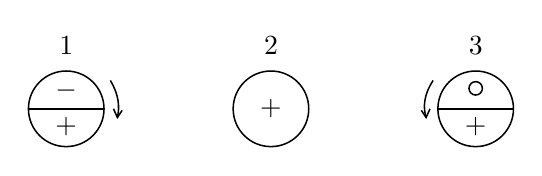
\begin{tikzpicture}[x=1cm,y=1cm,line width=.55pt]
\draw (0,0) circle (.48);\draw (-.48,0)--(.48,0);
\node at (0,.80){1};\node at (0,.23){$-$};\node at (0,-.23){$+$};
\draw (.56,.36) .. controls (.67,.18) and (.68,.02) .. (.65,-.11);
\draw (.60,.00)--(.65,-.11)--(.71,-.02);
\draw (2.6,0) circle (.48);\node at (2.6,.80){2};\node at (2.6,0){$+$};
\draw (5.2,0) circle (.48);\draw (4.72,0)--(5.68,0);
\node at (5.2,.80){3};\draw (5.2,.26) circle (.085);\node at (5.2,-.23){$+$};
\draw (4.66,.36) .. controls (4.54,.18) and (4.53,.02) .. (4.57,-.11);
\draw (4.51,-.02)--(4.57,-.11)--(4.62,.00);
\end{tikzpicture}\par\smallskip\textbf{Figur 1.}
\end{center}}
\newcommand{\EMThreeFigTwo}{%
\begin{center}
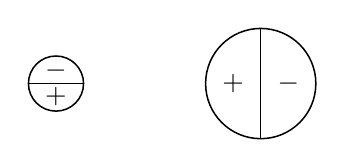
\begin{tikzpicture}[x=1cm,y=1cm,line width=.55pt]
\draw (0,0) circle (.35);\draw (-.35,0)--(.35,0);
\node at (0,.17){$-$};\node at (0,-.17){$+$};
\draw (2.6,0) circle (.7);\draw (2.6,-.7)--(2.6,.7);
\node at (2.25,0){$+$};\node at (2.95,0){$-$};
\end{tikzpicture}\par\smallskip\textbf{Figur 2.}
\end{center}}
\newcommand{\EMThreeFigThree}{%
\begin{center}
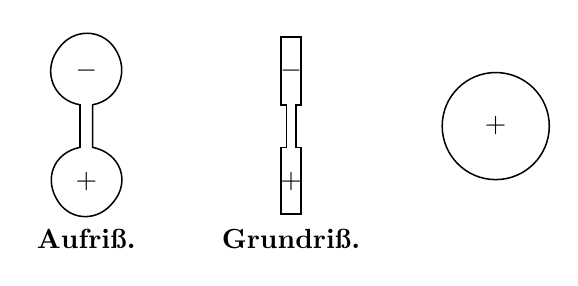
\begin{tikzpicture}[x=1cm,y=1cm,line width=.55pt]
\draw (-.08,.28)--(-.08,.82)
 .. controls (-.43,.88) and (-.57,1.27) .. (-.34,1.55)
 .. controls (-.16,1.79) and (.19,1.79) .. (.36,1.54)
 .. controls (.56,1.25) and (.41,.88) .. (.08,.82)
 --(.08,.28)
 .. controls (.43,.21) and (.57,-.15) .. (.34,-.42)
 .. controls (.15,-.66) and (-.18,-.66) .. (-.35,-.42)
 .. controls (-.55,-.13) and (-.42,.21) .. cycle;
\node at (0,1.25){$-$};\node at (0,-.16){$+$};
\node[below] at (0,-.64){\textbf{Aufriß.}};
\draw (2.47,1.68)--(2.73,1.68)--(2.73,.82)--(2.66,.82)--(2.66,.28)--(2.73,.28)--(2.73,-.57)--(2.47,-.57)--(2.47,.28)--(2.54,.28)--(2.54,.82)--(2.47,.82)--cycle;
\node at (2.6,1.25){$-$};\node at (2.6,-.16){$+$};
\node[below] at (2.6,-.64){\textbf{Grundriß.}};
\draw (5.2,.55) circle (.68);\node at (5.2,.55){$+$};
\end{tikzpicture}\par\smallskip\textbf{Figur 3.}
\end{center}}

\begin{center}
[2.]\par\medskip
\textbf{\textsc{Gauss} an \textsc{W. Weber}.}
\end{center}
\noindent . . . . . . . . . . . . . . . . . . . . .\par
\noindent\hspace*{\parindent}Vor einigen Tagen habe ich noch einmal versucht, Kohle in die galvanische Kette zu bringen. Meine alten (20 Jahre alten) Kohlen leiten gar nicht, während frisch ausgeglühete Kohlen einen vergleichungsweise gegen die 13000 Fuss lange Drahtkette (Multiplicator u. Indicator $6000+7000$) nur \textls[120]{kleinen} Widerstand darboten. Was mir aber besonders merkwürdig war, ist, dass \textls[120]{pulverisirte} Kohlen (frische) in einer breiten und dünnen Schicht zwischen zwei Metallplatten \textls[120]{gar nicht} leiten wollten. Ich weiss nicht, ob diess auch schon von andern bemerkt ist.

Erfreuen Sie, geliebter \textsc{Weber}, mich bald mit einem Briefe, am liebsten, mit der Nachricht Ihrer baldigen Rückkehr.
\par\medskip
\noindent\hspace*{\parindent}G[öttingen] den 10. Julius 1838.\hfill Ihr treuer C. F. G.\hspace*{\parindent}
\begin{center}
[3.]\par\medskip
\textbf{\textsc{Gauss} an \textsc{W. Weber}.}
\end{center}
\noindent\hspace*{\parindent}Die beiden für das Leipziger magnetische Observatorium und für Sie, mein theuerster Freund, bestimmten Exemplare der \textit{Observations etc.} sind mir nebst vielen andern zu vertheilenden, auf dem nicht ganz geraden Wege über Hamburg—Berlin—Leipzig von \textsc{Sabine} schon vor mehreren Wochen zugesandt: ich hatte bisher immer auf eine Gelegenheit zur Beförderung nach Leipzig gehofft, die sich aber nicht hat finden wollen.
\clearpage\SourceLeaf{180}\HistoricalHead{175}{R}{GAUSS AN W. WEBER.}
\noindent\hspace*{\parindent}Ihr Versuch, wodurch Sie die electrische Ungleichheit des Zinks und Kupfers direct erkennbar und messbar machen, hat mich sehr interessirt, und ich bin geneigt zu glauben, dass er der Anfangspunkt zu höchst wichtigen Fortschritten in dieser Lehre werden könnte. Ich fühle dabei aufs neue schmerzlichst, wie schön es gewesen sein würde, wenn ich mit Ihnen zusammen in diesem Felde hätte arbeiten können.

Rechnungen über die Vertheilung der Elektricität auf Ihrer zwei-metalligen Kugel lassen sich noch gar nicht machen, da es noch am Besten fehlt, nemlich an dem \textls[120]{präcisen} physikalischen Princip, wovon die Rechnungen ausgehen müssen. Diesem Princip vor allem müsste man auf die Spur zu kommen suchen; ist es einmal gefunden und befestigt, so wird es auf einmal in der Lehre Tag werden und neue Entdeckungen wie scheffelweise die Aepfel von einem schwerbelasteten Fruchtbaum uns von selbst in den Schooss fallen.

Wie die Elektricität auf einem leitenden (elektrisch homogenen) Körper sich vertheilt, dazu hat bekanntlich \textsc{Poisson} vor 30 Jahren die Grundgleichungen gegeben[*)],\begingroup\renewcommand{\thefootnote}{}\footnotetext{[*) S. D. \textsc{Poisson}, \textit{Mémoire sur la distribution de l'électricité à la surface des corps conducteurs} [1812] Mémoires de l'Institut, Paris 1811, S. 1—92, Second Mémoire [1813], ebenda (pte. 2), S. 163—274.]}\endgroup\ und die Folgen für mehrere interessante obwohl immer höchst einfache Fälle entwickelt. Nach \textsc{Voltas} Meinung, an die ich \textls[120]{vor Ihrem Versuche} niemals recht habe glauben können, vertheilt sich die Elektricität auf einem zusammengesetzten Körper anders als auf einem homogenen, so zwar, dass z. B. Zink mehr positive Elektricität enthält, wenn es mit Kupfer verbunden ist, als es haben würde, wenn es mit eben so geformtem Zink verbunden wäre. Aber es ist dies nicht viel mehr als Nichts wissen, so lange wir nicht das Quantitative dieses Mehr im Ganzen wie im Einzelnen klar überschauen können und dazu fehlt es zur Zeit noch an Allem. Aber Versuche werden schon auf die Spur führen können, wenn sie in grösster Mannichfaltigkeit und in möglichster Schärfe ausgeführt werden. Ich will zunächst nur ein Paar unreife Gedanken hersetzen:

1) Wenn Sie anstatt Ihrer Kugel aus Zink und Kupfer eine andere aus Metall, z. B. Zink, und Glas nehmen, so würde, deucht mir, jedenfalls ein ähnlicher Erfolg Statt finden, aber mit dem wesentlichen Unterschiede, dass letztere sich in Einerlei Sinn drehen würde, Sie mögen eine positive oder eine
\clearpage\SourceLeaf{181}\HistoricalHead{176}{L}{PHYSIK.\quad BRIEFWECHSEL.}
\noindent negative elektrisirte Kugel annähern, während nach Ihrer Mittheilung (von der mir gerade dies wie der wichtigste Punkt erschienen ist) bei Ihrer Kugel die Drehungen nach Maassgabe der Art der angenäherten Elektricität entgegengesetzt sind.

Ist diese Ansicht die richtige, so kann, deucht mir, eine solche Kugel dazu dienen, die Stärke der Elektrisirung der wirkenden Kugel zu messen. Diese Stärke der Elektrisirung wird wohl ziemlich schnell abnehmen, und in jedem Augenblicke ein Maass dafür zu haben, würde also ein wichtiges Bedürfniss befriedigen. Das Ganze sähe dann z. B. so aus:
\EMThreeFigOne
\noindent 1 die Zink-Kupferkugel, 2 die elektrisirte Kugel, 3 die Zink-Glaskugel. 1 und 3 sind zweckmässig bifilar aufgehängt und tragen Spiegel. Die Ablenkung von 3 wird dem Quadrate der Elektricitätsmenge von 2 proportional sein; wie wird sich aber die Ablenkung von 1 verhalten? Das eben sollen mannigfaltige Versuche lehren.

2) Mit sehr empfindlichen Beobachtungsmitteln würde sich vielleicht schon eine Ablenkung zeigen, wenn anstatt der elektrisirten 2 eine \textls[120]{nicht} elektrisirte Zink-Kupferkugel gebraucht wird, so
\EMThreeFigTwo
\noindent\hspace*{\parindent}Denn wenn es wahr ist, dass in der Berührung von Zink und Kupfer allezeit das erstere einen Überfluss positiver Elektricität gegen das letztere hat, so müssten sich doch zwei solcher Kugeln gleichsam wie polarisirte Magnete verhalten.

3) Sollte nicht anstatt einer aus Zink und Kupfer zusammengesetzten Kugel auch bloss ein metallisch verbundenes Paar Platten [sich] gebrauchen lassen? so aufgehängt:
\clearpage\SourceLeaf{182}\HistoricalHead{177}{R}{GAUSS AN W. WEBER.}
\EMThreeFigThree
\noindent\hspace*{\parindent}Mit Ihrer elektrisirten Kugel müssten Sie dächte ich diesem bifilar aufgehängten Scheibenpaar eben so gut eine Ablenkung ertheilen können wie Ihrer aus zwei Halbkugeln bestehenden Kugel, vermuthlich sogar eine stärkere, und solche Scheibenpaare lassen sich mit viel geringern Kosten herstellen.

Ich habe oben \textsc{Poissons} Arbeit von 1814[*)]\begingroup\renewcommand{\thefootnote}{}\footnotetext{[*) Gemeint ist die S. 175 in der Fußnote genannte Arbeit.]}\endgroup\ erwähnt. Die mathematische Kunst darin verdient alle Anerkennung, aber ich habe noch einige Zweifel, ob die physikalische Grundlage ganz richtig ist. Ich meine, ob diejenige Wirkung der Elektricitätselemente auf einander, welche dem Quadrat verkehrt proportional, hier \textls[120]{allein} im Spiel ist, oder ob nicht zugleich eine Art Molecularaction in Betracht gezogen werden muss, die viel mehr dabei wirkt, etwa so wie bei liquiden Flüssigkeiten die gegenseitige Gravitation der Theile $\left(\mathrel{::}\frac{1}{dd}\right)$ nur die zweite Rolle spielt neben nur in unmessbar kleinen Entfernungen wirkenden Kräften. Es ist dies in diesem Augenblick nur ein flüchtiger Gedanke, da das Gewicht der von \textsc{Poisson} beigebrachten \textls[120]{Versuche} mir jetzt nicht gegenwärtig genug ist. Bei einer blossen Wirkung $\mathrel{::}\frac{1}{dd}$ kann ich mir von der Ursache des \textsc{Volta}schen Fundamentalsatzes gar keine Vorstellung machen: bei einer Mitwirkung von Molecularkräften liesse sich schon eher etwas dem Kalkül zugängliches denken.

Doch es ist Zeit, diese unreifen Gedanken — die nur durch das Zutreten von \textls[120]{Erfahrungen} zur Reife kommen (oder als nichtig sich ausweisen) können — abzubrechen.

Mit den herzlichsten Empfehlungen an Ihre Herren Brüder, ingleichen an Herrn Professor \textsc{Möbius}
\par\medskip
\noindent\hspace*{\parindent}Göttingen 27. Januar 1844.\hfill\begin{tabular}[t]{@{}c@{}}stets ganz der Ihrige\\C. F. \textsc{Gauss}.\end{tabular}\hspace*{\parindent}
\par\medskip\noindent\hspace*{\parindent}. . . . . . . . . . .
\par\begin{center}\rule{.25\linewidth}{.4pt}\end{center}
\HistoricalFoot{XI\textsubscript{1}.}{23}
\clearpage\endgroup
